%
%

\multiproblem{linearop}{
  \begin{enumerate}
      \item Given homogeneity and additivity, prove that the principal of superposition is satisfied: $L(\alpha\mathbf{x_{1}}+\beta\mathbf{x_{2}})=\alpha L\mathbf{x_{1}}+\beta L\mathbf{x_{2}}$\\
You can prove bidirectional as linearity is equivalent to superposition.
\item Prove if an operator is linear or not:
\begin{enumerate}
\item $\int_{}^{}dx$ (integration) 
\item $\sin(x)$
\item $A\mathbf{x}$ where $A$ is a matrix.
\end{enumerate}
      
  \end{enumerate}
}

\multiproblem{diffeq}{
Consider $n$th-Order Linear Non-homogeneous Differential Equation:\\
\begin{align} 
{{y^{\left( n \right)}}\left( x \right) + {a_1}\left( x \right){y^{\left( {n - 1} \right)}}\left( x \right) +  \cdots  }
+ {{a_{n - 1}}\left( x \right)y'\left( x \right) + {a_n}\left( x \right)y\left( x \right)}=f(x)
\end{align}

The associated $n$th-Order Linear Homogeneous Differential Equation:
\begin{align} 
{{y^{\left( n \right)}}\left( x \right) + {a_1}\left( x \right){y^{\left( {n - 1} \right)}}\left( x \right) +  \cdots  }
+ {{a_{n - 1}}\left( x \right)y'\left( x \right) + {a_n}\left( x \right)y\left( x \right)}=0
\end{align}

Using the operator $Ly = f(x)$ we can re-write:\\

\begin{align} 
Ly={{y^{\left( n \right)}}\left( x \right) + {a_1}\left( x \right){y^{\left( {n - 1} \right)}}\left( x \right) +  \cdots  }
+ {{a_{n - 1}}\left( x \right)y'\left( x \right) + {a_n}\left( x \right)y\left( x \right)}
\end{align}

where $L$ is the $n$th-order linear operator.The coefficients $a_{1}(x)$ and  $a_{n}(x)$ can be either constants or functions $f(x)$. \\
Homogeneous Linear Differential Equations can be written in the form: $Ly=0$.\\
Non-homogeneous Linear Differential Equations: $Ly=f(x)$.\\

\begin{enumerate}
 \item  Show that for Second-Order Linear Differential Equation if $\alpha$ and $\beta$ are constants, then $L$ satisfies $L(\alpha y_{1}+\beta y_{2})=\alpha Ly_{1}+\beta Ly_{2}$\\\\
Proof (start):\\
Apply the operator $L$: $L(\alpha y_{1}+\beta y_{2})=a_{1}(x)\frac{{d}^2(\alpha y_{1}+\beta y_{2})}{{d}x^2}+...$\\
Regroup:..........\\
Get the final result: $\alpha Ly_{1}+\beta Ly_{2}$ 
 \item Show that if $y_{1}$ and $y_{2}$ are two solutions of a homogeneous linear differential equation Ly = 0, then every linear combination $y=\alpha y_{1} + \beta y_{2}$ with arbitrarily chosen coefficients is also a solution of $Ly = 0$.\\\\
Proof (start):\\
Suppose that $y_{1}$ and $y_{2}$ are two solutions of the differential equation. This means that $Ly_{1}=0.$\\
.............
\item The following Second-Order Differential Equation is given:
$\frac{\mathrm{d^2y} }{\mathrm{d} x^2} - y=0$\\
1. Show that $y_{1}=e^x$ and $y_{2}=e^{-x}$ are fundamental solutions for the above equation.
2. Using the superposition principle, come up with (a) any particular solution and (b) a general solution.

\item Linear differential equations can be represented in the form $Ly=f(x)$ where L is a linear operator.
Determine if a differential equation is linear or not:
\begin{enumerate}
\item $ \frac{\mathrm{d^2y} }{\mathrm{d} x^2} +y^2 =0$
\item $ \frac{\mathrm{d^4y} }{\mathrm{d} x^4} -y=1$
\item $ \frac{\mathrm{d^2y} }{\mathrm{d} x^2} -y \frac{\mathrm{dy} }{\mathrm{d} x} =0$
\end{enumerate}

\end{enumerate}

}

\multiproblem{nonhom}{

\begin{enumerate}

\item Suppose $y_{1}$ and $y_{2}$ are two solutions of a linear second order non-homogeneous differential equation $L(y) = f(x)$. \\
1. Show that their difference (not sum!!!) $y=y_{1}-y_{2}$ is the solution of the corresponding homogeneous equation $L(y) = 0$. \\
2. Show that all solutions for Second-Order Non-homogeneous Linear Differential Equations can be written as the sum of the complementary function (general solution of the associated homogeneous equation) and a particular solution of a non-homogeneous equation.\\

\item Using results in 2.3 and 2.5, come up with a general solution for the non-homogeneous differential equation:
$\frac{\mathrm{d^2y} }{\mathrm{d} x^2} - y=x$\\

\item Use the linearity to solve the following differential equation:
$\frac{\mathrm{d^2y} }{\mathrm{d} x^2} - y= 4e^{2x}+e^{-3x}$.\\

We can use linearity to split the problem into the solution of the two equations:\\
$\frac{\mathrm{d^2y} }{\mathrm{d} x^2} - y= e^{2x}$.\\
$\frac{\mathrm{d^2y} }{\mathrm{d} x^2} - y= e^{-3x}$.\\

Notice that the complementary function still needs to be worked out from the homogeneous equation.
The general solution will be in the form: \\
$y=y_{c}+4y_{1}+5y_{2}$


\end{enumerate}

}

\multiproblem{apps}{
Consider a pendulum with a rod of negligible mass attaching a weight of mass $m$ to the pivot, and with all mass
concentrated at the weight’s center of gravity at distance $l$ from the pivot. The motion, that is a repeated switching back and forth from side to side, is called an oscillation.

 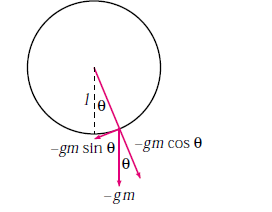
\includegraphics[scale=1]{pic1.png}
 \begin{enumerate}
  \item The following second order differential equation describes the movement of the pendulum: $\frac{{d}^2\theta}{{d}t^2}=-\frac{g}{l}\sin\theta$\\\\
Prove that it is a non-linear differential equation.\\
\item Recall Taylor Series of $\sin(x)$:
$\sin x = x - \large\frac{{{x^3}}}{{3!}}\normalsize + \large\frac{{{x^5}}}{{5!}}\normalsize - \large\frac{{{x^7}}}{{7!}}\normalsize +  \ldots  + \large\frac{{{{\left( { - 1} \right)}^n}{x^{2n + 1}}}}{{\left( {2n + 1} \right)!}}\normalsize \pm  \ldots$\\
Using approximation in Taylor Series, we-write the non-linear differential equation as a linear one and solve it. \\
Linearized pendulum equation is:..................\\
The solutions are the following:..................\\

The solutions of the linearized pendulum equation are examples of harmonic oscillations. Study of the nonlinear pendulum equation is the subject of the more advanced units.
 \end{enumerate}


}

\multiproblem{sys}{
Consider the system of linear differential equations with constant coefficients written in the matrix format:\\
$\frac{{d}\mathbf{x}(t)}{{d}t}=A\mathbf{x}$\\

Non-trivial solution can be written in the form:\\
\begin{align} 
\mathbf{x}=e^{\lambda t}\mathbf{v}
\end{align}
where $\mathbf{v}$ is an eigenvector and $\lambda$ is an eigenvalue. 
Notice that $\mathbf{v}$ should not be equal to zero.\\

\begin{enumerate}
 \item Show that the above formula is a solution for the system of linear differential equations.\\\\
General solution will be in the form:\\
\begin{align} 
\mathbf{x}=C_{1}e^{\lambda_{1} t}\mathbf{v_{1}}+ ...+C_{n}e^{\lambda_{n} t}\mathbf{v_{n}}
\end{align}
In order to find $\lambda$ we solve: $det(A-\lambda I)=0$. In order to find an eigenvector $\mathbf{v}$ for each $\lambda$ we solve: $(A-\lambda I)\mathbf{v}=0$

\item Solve the system of differential equations:\\
$\begin{cases}\frac{{d}x}{{d}t}=-2x+5y\\\frac{{d}y}{{d}t}=x+2y\end{cases}$

\item $\begin{cases}\frac{{d}x}{{d}t}=3x\\\frac{{d}y}{{d}t}=3y\end{cases}$
\end{enumerate}


}